\chapter{Kokoonpano}

Toisena merkittävänä alueena ketterän ryhmän hallinnallisissa haasteissa on ryhmäkokoonpanoon liittyvät haasteet, kuten muutokset ryhmässä ja kokoonpanon suunnittelu. Suunnittelun merkitys korostuu kokoonpanoon liittyvissä tehtävissä, kuten vastuunjaossa. On kuitenkin huomioitavaa, että suunnittelun merkitys nykyaikaisessa ohjelmistokehityksessä on muuttunut luonteeltaan perinteisiin malleihin, kuten vesiputousmalliin, nähden. Toisaalta puutteet suunnittelussa on kuitenkin yksi yleisimmistä ketterää toteuttavan ryhmän hallinnallisten haasteiden lähteistä \cite{7872736}. Beck et al. \cite{beck2001agile} määrittävät yhtenä ketteristä periaatteista, että muutokseen reagointi on tärkeämpää kuin suunnitelmassa pysyminen.

Tutkimuksessaan de Melo et al. \cite{DEOMELO2013412} toteavat ketterän ryhmän hallinnan olevan suurin vaikuttava tekijä tuottavuuteen. Tutkimus kartoitti merkittävimmät tuottavuuteen vaikuttavat tekijät, minkä myötä ne rajattiin ketterän ryhmän sisäisiin ja ulkoisiin haasteisiin kuvan 3.1 mukaisesti. Ryhmän sisäiset haasteet koostuvat suunnitteluvalinnoista sekä jäsenten vaihtuvuudesta ja niihin liittyvistä vaikutuksista, kun taas ulkoiset haasteet koostuvat useamman ryhmän välisestä yhteistoiminnasta.

% LISÄÄ TÄHÄN KAAVIO KOKOONPANOLLISISTA HAASTEISTA KUN VALMISTA
%\begin{figure}[t]
%\centering 
%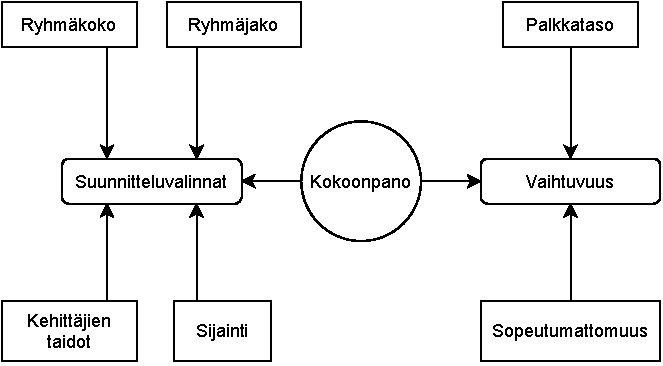
\includegraphics[width=1.0\textwidth]{template/figures/kokoonpanohaasteet.JPG}
%\caption{Kaavio kokoonpanohaasteista\label{fig:kokoonpanohaasteet}}
%\end{figure}

[\textbf{Katso löytyisikö seuraavaan kohtaan jotain lähteitä tukemaan vielä olettamusväitteitä, jotta olisi suorempaa viitettä}]


\section{Suunnitteluvalinnat}

[\textbf{Lisää Clapsin team role -pöhinät tänne!}]

Ryhmän suunnitteluvalinnat koostuvat ryhmäkoosta, ryhmäläisten taidoista, ryhmäläisten keskinäisestä sijainnista sekä ryhmäläisten jaosta \cite{DEOMELO2013412}. De Melo et. al \cite{DEOMELO2013412} tutkimuksesta on tulkittavissa, että haasteita kokoonpanoon tuottaa tässä kontekstissa muun muassa seuraavanlaiset tilanteet. Kokoonpanossa, jossa valtaosa ryhmäläisistä olisi osa-aikaisia työntekijöitä keskinäinen keskittyminen projektiin voisi olla heikkoa perustuen tutkimuksen toteamukseen tapauksesta, jossa täyspäiväjäsenillä on parempi keskittyminen. Ryhmän monipuolisuus kokemusten ja taitojen osalta on todettu hyödylliseksi siten, että kokeneilla on laaja kokemuskirjo, kun taas vähemmän kokeneet ryhmäläiset ovat yleensä joustavampia. Ryhmän kokoon liittyen on todettu, että pienemmän ryhmän koordinaatio (erityisesti kommunikoinnin osalta), konfliktinhallinta, sitoutuminen sekä vastuuntunto ovat paremmalla tasolla kuin suuremmissa ryhmissä. Suuremman ryhmäkoon on todettu monimutkaistavan ryhmätyöskentelyä esimerkiksi siten, että useampi kehittäjä saattaa heikentyneen kommunikaation johdosta työskennellä tietämättään samojen asioiden parissa. Tästä aiheutuu ylimääräistä päällekkäistä työskentelyä, jonka myötä ryhmän tuottavuus heikentyy. Ryhmän sijainnin on todettu vaikuttavan erityisesti vaatimusmäärittelyn ja suunnittelun toteutukseen siten, että paikallisessa ketterässä ryhmässä ne ovat huomattavasti helpompia. Paikallisen ryhmän kommunikointi sekä koheesio ovat myös parempia kuin esimerkiksi maantieteellisesti hajautetussa ryhmässä.

\section{Vaihtuvuus}

Ryhmän jäsenten vaihtuvuus on toinen ryhmän sisäistä haasteista. Vaihtuvuudeksi de Melo et al. \cite{DEOMELO2013412} määrittävät sekä aiemman kehittäjän lähtönä ryhmästä että uuden kehittäjän liittymisenä ryhmään. Vaihtuvuus aiheuttaa organisaatiolle monenlaisia kustannuksia, kuten irtisanoutumiseen, rekrytointiin sekä perehdyttämiseen liittyen. Lisäksi kehitysryhmä työskentelee vaihtuvuuden aikana astetta pienemmällä teholla johtuen joko pienemmästä määrästä kehittäjiä ryhmässä tai uuden ryhmäläisen perehdyttämisestä. Eräässä tutkimuksen tapauksista uusi ryhmäläinen  Tutkimuksessaan de Melo et al. määrittävät vaihtuvuuden tekijöiksi palkkatason sekä kehittäjän sopeutumattomuutena ryhmään. Sopeutumattomuuden on arvioitu johtuvan muun muassa oma-aloitteisuuden ja sitoutumisen puutteesta, epäsopivasta personaallisuudesta sekä ryhmän sisäisistä erimielisyyksistä. Viimeisestä on tulkittavissa, että haasteet kommunikoinnissa voivat aiheuttaa kokoonpanollisia haasteita. 

Vaikka vaihtuvuuden voi tulkita aiheuttavan kokoonpanollisia haasteita, niin sen on todettu vaikuttavan positiviisesti tilanteessa, jossa ryhmään liittyy uusi kehittäjä \cite{DEOMELO2013412}. Uudet ryhmäläiset saattavat tuoda uusia ideoita, ratkaisuja ja yleisesti ottaen energiaa ryhmään. Toisaalta vaihtuvuuden negatiivisia vaikutuksia on lukumäärällisesti enemmän ja ne voidaan jakaa pidentyneeksi tuotantoajaksi lyhyellä aikavälillä, oleellisen tiedon menettämisenä poistumisen yhteydessä sekä lisäkustannuksina. 

De Melo et al. \cite{DEOMELO2013412} kiteyttävät ketterän ryhmän perustuvan yksilöihin ja ryhmätyöskentelyyn. Oikeilla menetelmillä toteutettuna kommunikaation ja yhteistyöskentelyn on todettu parantuvan. Tutkimus korostaa ketterien menetelmien prosessia tehostavia työskentelytapoja, kuten pariohjelmointia, päivittäistapaamisten ja yhteisistuntojen pitämistä. Kaiken kaikkiaan ketterien menetelmien oikeanlaisen ja tarpeeksi laajan toteutuksen on todettu vähentävän vaihtuvuuden riskiä. Toisaalta on huomioitava, että vaihtuvuus on varsin yleinen ilmiö.

\section{Useamman ryhmän yhteistoiminta}

Tutkimuksessaan de Melo et al. \cite{DEOMELO2013412} toteavat ketterän ryhmän tuottavuuden koostuvan ryhmän sisäisistä ja ulkoisista tekijöistä. Ryhmän ulkoiset tekijät rajautuvat useamman ryhmän väliseen koordinaatioon. Ryhmien välisen koordinoinnin haasteita aiheuttavat sitoutumisen puute sekä epäsopivat koordinointisäännöt ryhmien välillä. Haasteiden on todettu aiheuttavan suuntausvirheitä ja pahimmillaan ketteryyden rikkoutumisen. Esimerkkinä suuntausvirheestä toimii tilanne, jossa ryhmän työskentely riippuu toisen ryhmän tuloksista, eivätkä ryhmät työskentele samassa tahdissa. Tällöin syntyy tilanteita, joissa toisesta ryhmästä riippuva ryhmä joutuu odottamaan tai hidastamaan tahtiaan merkittävästi.